
\documentclass{bmcart}


\usepackage[utf8]{inputenc} %unicode support

\usepackage{graphicx}
\usepackage{bm}
\usepackage{subfigure}
\usepackage{multirow}
\usepackage{algorithm}
\usepackage{algorithmic}
\usepackage{array}
\usepackage{subfigure}
\usepackage{mathrsfs}
\usepackage{epstopdf}
\usepackage{amsmath}

\startlocaldefs
\endlocaldefs


%%% Begin ...
\begin{document}

%%% Start of article front matter
\begin{frontmatter}

\begin{fmbox}
\dochead{Research}

\title{Consistent Multiple Nonnegative Matrix Factorization with Hierarchical Information for Gene Functional Modules Mining}


\author[
   addressref={aff1},                   % id's of addresses, e.g. {aff1,aff2}
   corref={aff1},                       % id of corresponding address, if any
   noteref={n1},                        % id's of article notes, if any
   email={jane.e.doe@cambridge.co.uk}   % email address
]{\inits{JE}\fnm{Jane E} \snm{Doe}}
\author[
   addressref={aff1,aff2},
   email={john.RS.Smith@cambridge.co.uk}
]{\inits{JRS}\fnm{John RS} \snm{Smith}}


\address[id=aff1]{%                           % unique id
  \orgname{Department of Zoology, Cambridge}, % university, etc
  \street{Waterloo Road},                     %
  %\postcode{}                                % post or zip code
  \city{London},                              % city
  \cny{UK}                                    % country
}
\address[id=aff2]{%
  \orgname{Marine Ecology Department, Institute of Marine Sciences Kiel},
  \street{D\"{u}sternbrooker Weg 20},
  \postcode{24105}
  \city{Kiel},
  \cny{Germany}
}



\begin{artnotes}
%\note{Sample of title note}     % note to the article
\note[id=n1]{Equal contributor} % note, connected to author
\end{artnotes}

\end{fmbox}% comment this for two column layout

\begin{abstractbox}

\begin{abstract} % abstract
\parttitle{Motivation} %if any
An increasing amount of genome-phenome association data, has provided us an unprecedented chance to globally explore the underlying genetic mechanisms and understand the regularization between genes and diseases with a deeper sight perspective. Gene clustering, which reveals the interactions between genes and help researchers to identify candidate genes as drug targets et,al., has always been a significant and valuable problem by using genome-phenome association data. Nevertheless, the hierarchical structure of phenotype ontology has been rarely leveraged by previous gene clustering studies, the properties of genes, diseases and their relationships has not been fully explored, which may result in missing the chance to discover the crucial fact in biology. Thereby It is challenging to utilize this neglected hierarchical character of phenotype ontology to gain understanding of biological system.\\
\textbf{Results:}
We propose a novel method, Consistent Multiple Nonnegative Matrix Factorization (CMNMF), to utilize the hierarchical structure of phenotype ontology to cluster genes in factoring genome-phenome association data on mouse. The CMNMF method, constrains the gene cluster to remain consistent while interacting with different phenotype ontology levels in decomposing the genome-phenome association matrix, meanwhile it restricts the similarity of phenotype pairs to satisfy the hierarchical structure. The performance of our proposed method and other baselines (including NMF, K-means, KK-kernel, HAC) are evaluated on $F_1$ measure and Gene Ontology similarity measure. The results show the effectiveness of our proposed method compared with other baselines. Additionally, we conduct the regularized Consistent Multiple Nonnegative Matrix Factorization(R-CMNMF) on gene clustering, R-CMNMF beats other baselines as well. \\
Our work explores the crucial impact of hierarchical structure of phenotype ontology in gene clustering, and we show our proposed method outperforms baselines in both unsupervised and supervised manner, which provides a new perspective to conduct research on biological data exploration.\\
\textbf{Availability:} Github\\
\textbf{Contact:} {name@bio.com}{name@bio.com}\\
\parttitle{Second part title} %if any
Text for this section.
\end{abstract}


\begin{keyword}
\kwd{sample}
\kwd{article}
\kwd{author}
\end{keyword}


\end{abstractbox}
%
%\end{fmbox}% uncomment this for twcolumn layout

\end{frontmatter}


\section*{Introduction}
With the development of technology, biomedical researchers has collected a large amount of valuable biological data by these years, especially the genome-phenome association data on mouse, whose research achievement may transfer to men's disease study, it is of great significance for drug development and disease treatment for humans. Thereby it is necessary and essential for researchers to have a deeper sight investigation on mouse data. The international database resources such as Mouse Genome Informatics(MGI), Kyoto Encyclopedia of Genes and Genomes(KEGG) et al. provide more and more multiple types of mouse biological data. However, how to integrate and utilize those data in a effective way to discover the underlying patterns and biological mechanism is still a challenging issue, which has drawn growing attention in the literature.

It is well known that genes in mammal genomes are usually organized into groups functionally associate with phenotype groups(ref).Identification of modules of functionally related genes is a crucial first step towards dissecting the regulatory circuitry underlying biological processes. Co-regulated or functionally related genes are likely to reveal themselves by associations with different diseases. These modules may provide clues about the main biological processes associated to different physiological states and provide guidance for candidate genes of genetic diseases.

Phenotypes, is the composite of an organism's observable characteristics or traits, results from the expression of an organism's genes as well as the influence of environmental factors and the interactions between the two. (1,2). The key to achieving desired gene modules such as favorable disease treatment outcomes lies in the understanding of the relation between phenotypes and the biological roles of genes (3,5). Phenotype ontology was created to serve as a standardized vocabulary of phenotypic abnormalities that have been seen in diseases, can be used as a computational representation of phenotype knowledge based upon a hierarchical structure(ref). This kind of structure provides researchers extra information about the relationships between phenotype pairs. Whereas ,as far as we know, the hierarchical structure of phenotype ontology has not been utilized for gene module identification, the phenotype ontology in different levels reflects underlying associations while interacting with disease genes. With taking advantage of this character, it gives us a new perspective to explore the patterns behind the biological data.

Much research studies have been conducted on integration of multiple sources of biological data to mine the hidden patterns and the relationships between distinct data sources. Some procedures based on gene expression profiles, seeking to map different experimental data types, such as gene expression, miRNA expression, and copy number variation to a common space of known biological pathways or sets(Khatri et al.,2012; Mitrea et al.,2013). (Zhang et al., 2011) focuses on integrating multiple type genomic data to identify microRNA-gene regulatory modules for cancers. Extended Dirichlet mixture model(Lock and Dunson,2013) and principal component analysis(Lock et al., 2013) make the distinction between common and distinct effects across sources. Some studies incorporated clinical phenotype data to increase the ability of identifying new disease-associated genes(Hwang et al., 2012; Lage et al., 2007; Li and Patra, 2010; Vanunu et al., 2010; Wu et al., 2008, 2009)("Phenome-driven disease genetics prediction toward drug discovery"), a key assumption in these methods is that  similar disease phenotypes reflect overlapping genetic causes(Houle et at.,2010).("Phenome-driven disease genetics prediction toward drug discovery"). Because some data contains specific structures behind it, thus some structure based methods are proposed and all achieve good results. In the collaborative recommendation task, some grouping strategies based on structure information are proposed, such as grouping users by social networks, grouping items by defined hierarchy or grouping both of them (SoRec,HMF,HGMF). HPMF focuses on predicting missing traits for plants which incorporates hierarchical phylogenetic information into matrix factorization (HPMF). The results of these methods demonstrate that considering auxiliary structured information can bring a better performance.

In this study, we developed a novel NMF based approach consistent multiple nonnegative matrix factorization (CMNMF) to combine structured phenotype ontology data on mouse disease phenotype to predict disease-associated gene modules. The key ideas of our method are that the same gene should be active in the same modules when interacting with phenotypes from different levels of the hierarchical phenotype ontology  and the similarity of phenotype pairs, which has parent-child relationships, should keep high in the hierarchical structure. To demonstrate the approach, we conduct our proposed method on a series of measurements with other baselines on gene clustering task in an unsupervised way, the performance of our CMNMF on $F_1 measure$, $Rand index$, $Jaccard index$, and $GO Score$ outperform other baselines, including K-means, PCA K-means KernelK-means, HAC, NMF, LDA. Besides, we conduct regularized CMNMF(R-CMNMF) on gene classification, the AUC score demonstrates the advantages of CMNMF over SVM, LP.

The remainder of the paper is organized as follows. We present our consistent multiple nonnegative matrix factorization framework in Section 2. Section 3 reports some experiments and discussions. Followed with conclusion and future work in section 4.


\section*{Method}
In this section, we describe our framework for the consistent multiple non-negative matrix
factorization with hierarchical information of genome-phenome association data to identify gene modules.
We designed an objective function with three components. The first and second components are based on non-negative genome-phenome association data with respect to distinct level phenotype ontologies. The third one considers the effects of interactions from phenotype ontology. By optimizing this objective function, we obtain a consistent decomposition of two genome-phenome association matrix, which reveals gene functional modules inherent in genome-phenome association data jointly.

\subsection*{Data Preparation}
In this study, we evaluate the proposed CMNMF and baseline methods on MGI mouse gene-phenotype ontology association data. The mouse gene-phenotype ontology associations are extracted from file ``MGI\_Geno\_Disease.rpt'' (March-2015) downloaded from MGI \footnote[1]{ftp://ftp.informatics.jax.org/pub/reports/MGI\_Geno\_Disease.rpt}, in which 5894 phenotype-gene associations at level 4 and 6817 associations at level 5 are kept. 2144 ontology terms at level 4 (parent level) and 2719 ontology terms at level 5 (child level)  are selected from the 10748 MP terms in the OBO file. 2866 hierarchial mapping relations between phenotypes in level 4 and level 5 are kept as $M$.

To evaluate the performance, we collected 288 pathways from KEGG as the ``ground truth''. Genes in a signal pathway can be considered as a gene functional module (or a gene cluster).

\begin{table}[!t]
%\processtable{Summary of notations.\label{Tab:01}} {
\begin{tabular}{ll}
    \hline
    % after \\: \hline or \cline{col1-col2} \cline{col3-col4} ...
    Notations & Explanations\\
    \hline\hline
    $A_1$ & genome-phenome association matrix with phenotype\\
    & ontology from level 4\\
    $A_2$ & genome-phenome association matrix with phenotype\\
    & ontology from level 5\\
    $m$ & Number of disease genes\\
    $k$ & Number of gene clusters(e.g. classes)\\
    $G$ & Gene cluster membership\\
    $P$ & Phenotype cluster membership\\
    $M$ & Phenotype ontologies relationship\\
    \hline
  \end{tabular}
%}{}%This is a footnote
\end{table}

\subsection*{Problem formulation}
The notations and definitions used in the article are specified in Table(\ref{Tab:01}).
We denote $A_{(m \times n)}$ a binary gene-phenotype association matrix by $m$ genes and $n$ phenotypes, where $A_{ij}$ is set with 1 for known association and 0 otherwise. The goal of factorizing matrix $A$ based on NMF(Lee and Seung,1999) is to derive gene functional clusters based on gene-phenotype associations. The loss of it can be defined as:
\[min _{P,G} ||A-GP||^{2}_{F}\]
Where $G$ and $P$ denotes gene clusters and phenotype clusters , respectively. The notation $||\bullet||_F$ means the Frobenius norm of a matrix.

Based on multiplicative update rules(Lee and seung,2000), we can get a non-negative solution of $G$ and $P$. The elements of $G$ can be interpreted as latent modules associated with genes, thus a couple of clusters of genes are achieved with a good interpretation on NMF.
However, the NMF method in this form has not taken the hierarchical mapping information of phenotype ontology into consideration. To address this problem, we design a loss function with two aspects for formulating the loss with hierarchical information of phenotype ontologies.

1)The first aspect is a consistent constraint on gene cluster, the reason is intuitive, one gene interacts with a child phenotype ontology, it should interact with the child ontology's parent phenotype ontology, because parent phenotype ontologies are generalization of child phenotype ontologies, the child phenotype ontologies are specification of parent phenotype ontologies. (e.g. xxxxx)Fig. 1(a) shows The gene clustering results on general and specific phenotype ontology level, on which we put a consistent constrain.\\
2)The second component is a hierarchical mapping constraint with phenotype ontologies from parent level and child level. (Fig. 1(b)). With it, the clusters of phenotype ontologies from different level should also be consistent. By optimizing these two components, a CMNMF (Consistent Multiple Non-negative Matrix Factorization) algorithm is proposed to obtain consistent gene cluster.



\subsection*{Loss Functions for Penalizing Inconsistence}

Motivated by the consistent assumption, we extract phenotype ontologies from two adjacent levels, and denoted them as $P_{1}$ and $P_{2}$. Correspondingly, two gene-phenotype association matrices $A_{1}$ and $A_{2}$ are extracted according to two extracted sets of phenotype ontologies and all genes. We assume that the factorizations on  $A_{1}$ and $A_{2}$ for the same gene set should be consistent, although the gene are annotated by phenotype ontologies from parent levels and child levels, respectively. In our work, factorized $G_{1}$ and $G_{2}$ should be same. Hence, we use the same $G$ in two terms of matrix factorization. The following quadratic function can be used to model the first loss:

\begin{equation}
{L_C} = \mathop {\min }\limits_{G,{P_1},{P_2}} \left\| {{A_1} - G{P_1}} \right\|_F^2 + \alpha \left\| {{A_2} - G{P_2}} \right\|_F^2,
\end{equation}

where $\alpha$ is a parameter to balance the factorization error from different levels.

For the hierarchical mapping constraint on phenotype ontologies from parent level and child level, loss function in Eq. is used to encourage the consistence between phenotype clustering in parent level and child level.

\begin{equation}
{L_H} = \sum\limits_{ij} {{M_{ij}}} {(p_1^{(i)})^T}p_2^{(j)} = tr({P_1}MP_2^T),\
\end{equation}
where matrix $M$ denotes the hierarchical mapping relations between phenotype ontologies from different levels.  The $M_{ij}=1$, if phenotype $i$ and phenotype $j$ have a parent-child relationship, otherwise 0. We enforce hierarchical mapping constraints by maximizing the mapping between the phenotype ontologies in gene-phenotype network $A_{1}$ and $A_{2}$.

\subsection*{Regularization by Sparse Constraint}
Since the known gene-phenotype associations are sparse and only cover a part of genes and phenotypes, the regularization with $L_2-norm$ is proposed to control the sparseness of $G$, $P_1$ and $P_2$. The term ${\lambda _1}\|G\|_F^2$ limits the shareness of gene in different gene functional modules. The term ${\lambda _2}(\| {{P_1}}\|_F^2+\|P_2\|_F^2)$ also encourages the sparsity of phenotype clusters. Finally, the loss function of regularized CMNMF with sparse constraint and non-negative constraint is listed as follows:
\begin{equation}\label{S-CMNMF}
\begin{split}
\mathop {\min }\limits_{G,{P_1},{P_2}}
&\left\| {{A_1} - G{P_1}} \right\|_F^2 + \alpha \left\| {{A_2} - G{P_2}} \right\|_F^2 - \gamma tr({P_1}MP_2^T)\\
&{\rm{ + }}{\lambda _1}\left\| G \right\|_F^2{\rm{ + }}{\lambda _2}(\left\| {{P_1}} \right\|_F^2{\rm{ + }}\left\| {{P_2}} \right\|_F^2)\\
&\mathrm{s.t. }\qquad {\rm{  G}} \ge {\rm{0, }}\quad{{\rm{P}}_1}{\rm{, }} {{\rm{P}}_2} \ge 0
\end{split}
\end{equation}
where $\alpha ,\gamma ,{\lambda _1},{\lambda _2}$ are parameters to balance the trade of each component.
\subsection*{supervised CMNMF}
The loss function:
\begin{equation}\label{S-CMNMF}
\begin{split}
\mathop {\min }\limits_{G,{P_1},{P_2}}
&\left\| {{A_1} - G{P_1}} \right\|_F^2 + \alpha \left\| {{A_2} - G{P_2}} \right\|_F^2 +\beta\left\| {G - {G_0}}\right\|_F^2\\
&- \gamma tr({P_1}MP_2^T){\rm{ + }}{\lambda _1}\left\| G \right\|_F^2{\rm{ + }}{\lambda _2}(\left\| {{P_1}} \right\|_F^2{\rm{ + }}\left\| {{P_2}} \right\|_F^2)\\
&\mathrm{s.t. }\qquad {\rm{  G}} \ge {\rm{0, }}\quad{{\rm{P}}_1}{\rm{, }} {{\rm{P}}_2} \ge 0
\end{split}
\end{equation}
When fixing $P_1$ and $P_2$,the partial derivative of $L$ with respect to $G$ is:

\begin{equation}\label{S-CMNMF-gradient}
\begin{split}
\frac{\partial{L}}{\partial{G}}=
&-2(A_1{P_1^T} - G{P_1}{P_1^T})-2\alpha(A_2{P_2^T} - G{P_2}{P_2^T})\\
&+2\beta(G-G_0)+2\lambda_1G+\phi
\end{split}
\end{equation}
Using the Karush-Kuhn-Tucher(KKT) conditions, $\phi_{ij}G_{ij}=0$, we can get the following updating rule for G:
\begin{equation}\label{updating_G}
\begin{split}
G_{ij}\leftarrow G_{ij}
\frac{(A_1P_1^T+\alpha A_2P_2^T+\beta G_0)_{ij}}
{(GP_1P_1^T+\alpha GP_2P_2^T+\lambda_1G+\beta G)_{ij}}
\end{split}
\end{equation}
Similarly, when fixing G, the partial derivative of $L$ with respect to $P_1$ and $P_2$ are:
\begin{equation}\label{derivate_P}
\begin{split}
&\frac{\partial{L}}{\partial{P_1}}=
-2(G^TA_1-{G^TGP_1})-\gamma P_2M^T +2\lambda_2P_1+\phi\\
&\frac{\partial{L}}{\partial{P_2}}=
-2\alpha(G^TA_2-{G^TGP_2})-\gamma P_1M +2\lambda_2P_2+\Omega
\end{split}
\end{equation}
then, we can get the updating rules for $P_1$ and $P_2$:
\begin{equation}\label{updating_P}
\begin{split}
&(P_1)_{ij}\leftarrow (P_1)_{ij}
\frac{(G^TA_1+\frac{1}{2}\gamma P_2M^T)_{ij}}
{(G^TGP_1+\lambda_2P_1)_{ij}}\\
&(P_2)_{ij}\leftarrow (P_2)_{ij}
\frac{(\alpha G^TA_2+\frac{1}{2}\gamma P_1M)_{ij}}
{(\alpha G^TGP_2 + \lambda_2P_2)_{ij}}
\end{split}
\end{equation}
\subsection*{The CMNMF Algorithm}
To minimize the loss function in Eq. , we have developed an algorithm CMNMF that can optimize the objective function iteratively by fixing one variable alternatively. As in the original NMF model, the cost function (3) is not convex in $G$ and $P$ jointly, but it is convex in $G$ for fixed $P_1$ and $P_2$, vice versa. the Lagrange multiplier method can be applicable here to give an iterative algorithm to guarantee the algorithm to converge to a local minima \cite{document_cluster_NMF}. Algorithm 1 describes the iterative algorithm for the CMNMF model.

\section*{Experiments and Analysis}
Our method is demonstrated on simulated gene-phenotype association matrixes at first by comparing the difference of conventional NMF and proposed CMNMF. We then execute CMNMF and four baseline methods on MGI mouse gene-phenotype ontology associations for mining mouse gene functional modules. Moreover, the evaluation of clustering results and parameter tuning are performed. Finally, gene ontology enrichment analysis by DAVID is adopted to evaluate the biological significance of mined gene modules.

\subsection*{1 CMNMF on Simulated Data}
We generated gene-phenotype association matrixes $A_1$, $A_2$ and hierarchical mapping relations $M$ to illustrate the usage of the hierarchical information. Fig.\ref{fig:simulate_data}(a) describes the structure of the simulated data in which genes are assigned into three groups. For each group, there are two genes associating with phenotypes in the child level and another gene associating with the parent phenotypes. The task is to cluster the three genes into a same group. Due to the third gene doesn't have any associated phenotypes in the same level with that another two genes associate with, neither on $A_1$ nor on $A_2$ can NMF group the third gene into a same cluster with another two as shown in Fig.(\ref{fig:simulate_data})(b-1) and Fig.(\ref{fig:simulate_data})(b-2).
\begin{figure}
  \centering
  \begin{minipage}{.4\linewidth}
  \centering
    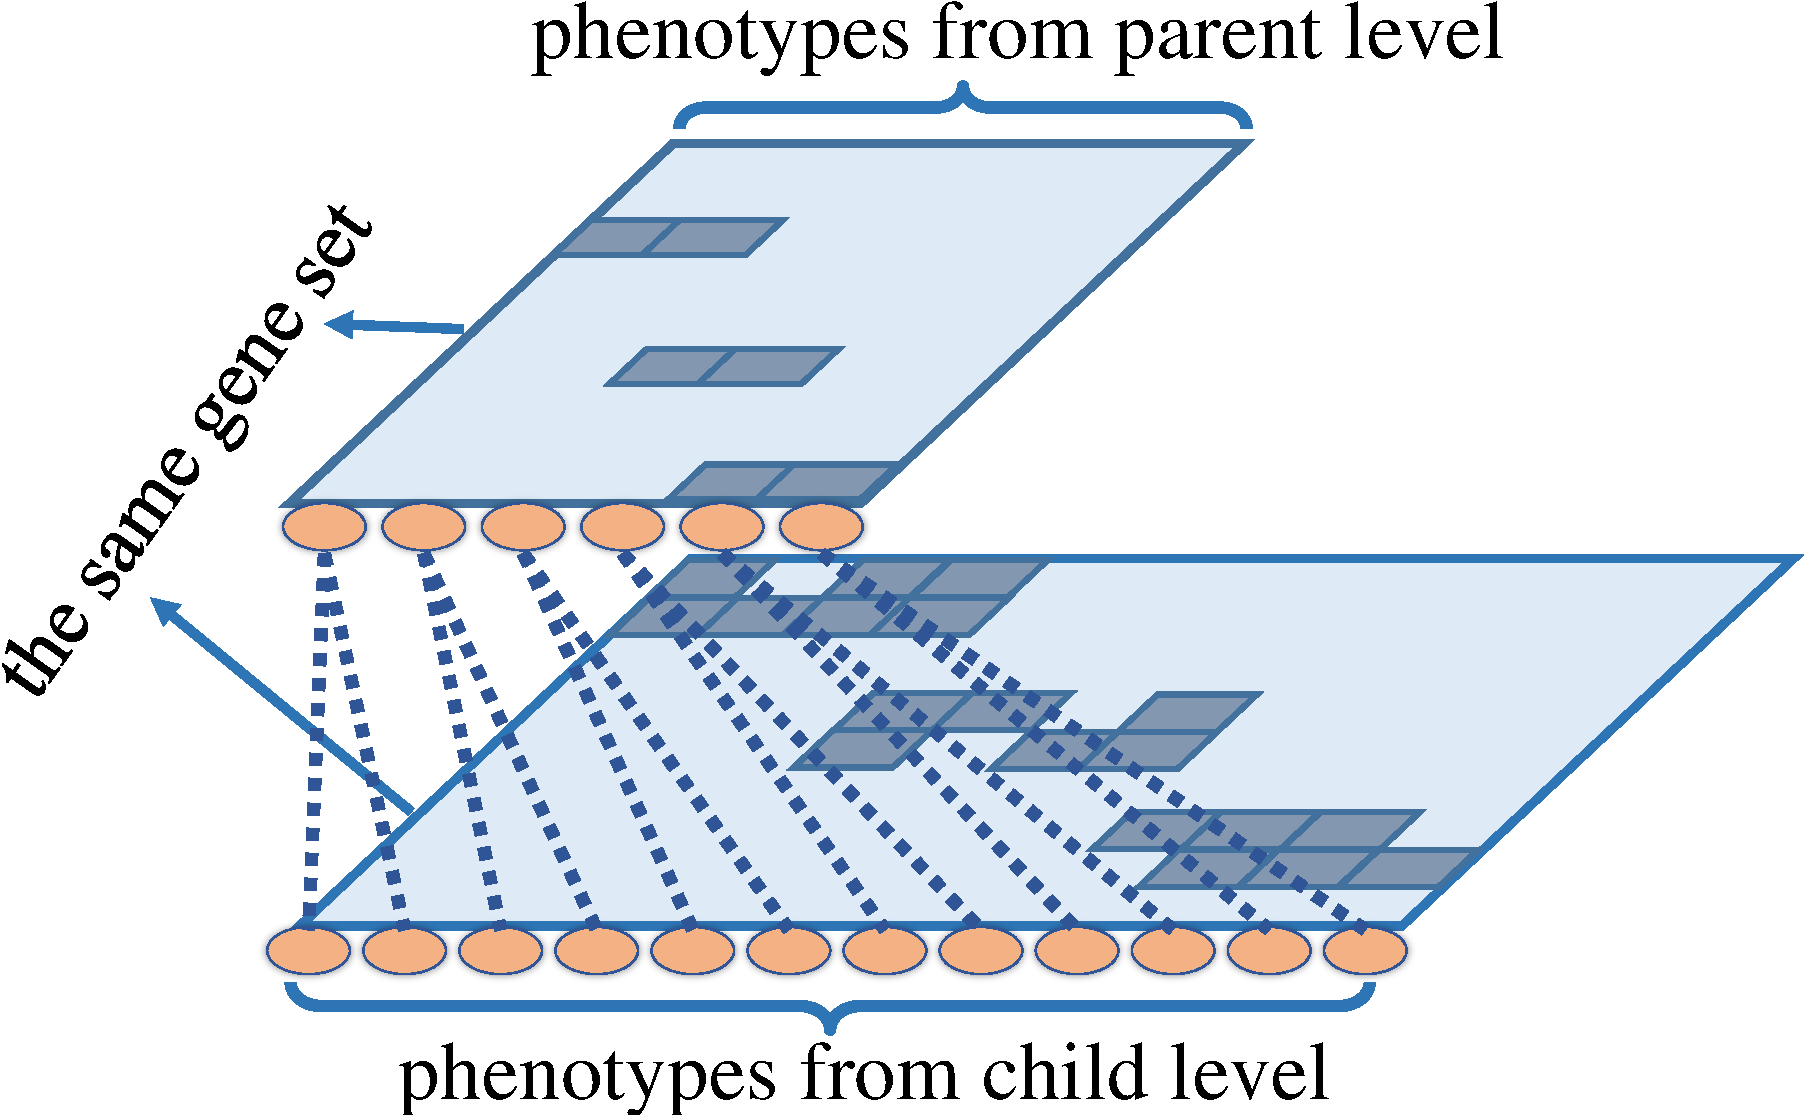
\includegraphics[width=\linewidth]{fig/simulate_data.pdf}
    \centerline{(a)}
  \end{minipage}
  \begin{minipage}{.4\linewidth}
   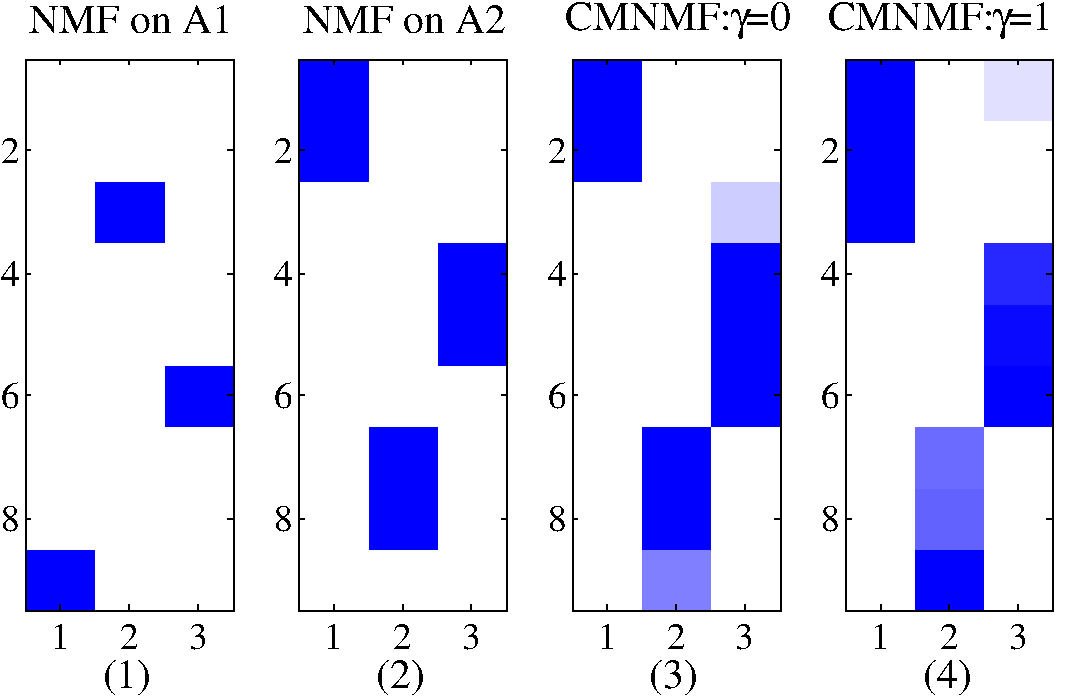
\includegraphics[width=\linewidth]{fig/simulate_result.pdf}
    \centerline{(b)}
  \end{minipage}
  \caption{(a)Hierarchical structure of simulated data, (b) Performance of CMNMF and NMF under different conditions: (b-1) Cluster result of NMF on parent level, (b-2) Cluster result of NMF on child level, (b-3) Cluster result of CMNMF($\gamma$=0), (b-4) Cluster result of CMNMF($\gamma$=1)}
  \label{fig:simulate_data}
\end{figure}

To analyze how the two proposed constraints work, CMNMF is applied to the simulated data to cluster the genes. We first set the parameter $\gamma$ which controls the effect of hierarchical constraint on CMNMF to zero. As shown in Fig.\ref{fig:simulate_data}(b-3), combing information from two levels and restricting the cluster results of genes to remain consistent indeed help improve the performance. But there still exists little misclassification (the third gene in the first group is wrongly assigned to the second group). When introducing the hierarchical constraint ($\gamma$=1) to the model, the CMNMF method groups all the genes into the correct clusters (See Fig.\ref{fig:simulate_data}(b-4)), which demonstrates that the two constraints working together can get the best performance. The reasons for the performance improvement are that with the consistent constraint, CMNMF can incorporate information from two levels and take advantage of the complement characteristic of information from different levels to overcome the shortcoming of lacking enough information from only one level and the hierarchy constraint can help restrict cluster results according with the structure of data which narrows the range of solution space so that we can get a better solution.

\subsection*{2 Functional gene module similarity analysis}

\subsection*{3 Comparison with Baseline Methods by Mining Gene Modules}
CMNMF is executed to mine gene functional modules and it is compared with the following clustering methods, K-Means, HAC (Hierarchical Agglomerative Clustering) \cite{HAC}, NMF and HMF(Hierarchical Matrix Factorization) \cite{HMF}. To be fair, all matrix factorization-based methods are implemented with sparse and non-negative constraints. We measured the performance by the Jaccard coefficient \cite{cluster_survey}. Higher coefficient indicates better clustering result.

Parameters are tuned by cross-validation for all the competitive methods respectively. For all matrix factorization methods, the balancing parameter of sparse constraints on gene clusters $\lambda_1$ and phenotype clusters $\lambda_2$ are set by the grid \{0.001,0.01,0.1,1,10,20\}. For CMNMF, the weight of factorization on child level $\alpha$ is set from 0.1 to 0.9 with an interval of 0.2 and 1 to 9 with an interval of 2, $\gamma$ is set by the range \{0.0001,0.001,0.01,0.1,1\}. The number of modules k is picked to be 300 for all methods, approximating to the number of KEGG mouse pathways. Initial values of $G$ and $P$ (or $P_1$ and $P_2$) are randomized with value between 0 to 1.

The clustering results are column-normalized by using z-score, and the $G_{ij}$ will be set as 0 if it is less than $3\sigma$. All the methods are repeated ten times with different initial values and average Jaccard coefficients are reported in Fig.\ref{fig:jaccard}. Note that the proposed method performs better than other methods except HAC as shown in Fig.\ref{fig:jaccard}(a). But the range of gene clusters size of HAC is much larger than other methods as shown in Fig.\ref{fig:jaccard}(b). In fact, HAC puts 76.5\% of genes into one cluster and the other clusters share the left genes which brings it a better Jaccard coefficient, but it cannot help to identify significant gene functional modules. Additionally, the standard deviations of all the methods are small, which demonstrates that these methods including our CMNMF are insensitive to the initial values (Fig.\ref{fig:jaccard}(a)).
\begin{figure}
  \centering
  \begin{minipage}{.45\linewidth}
    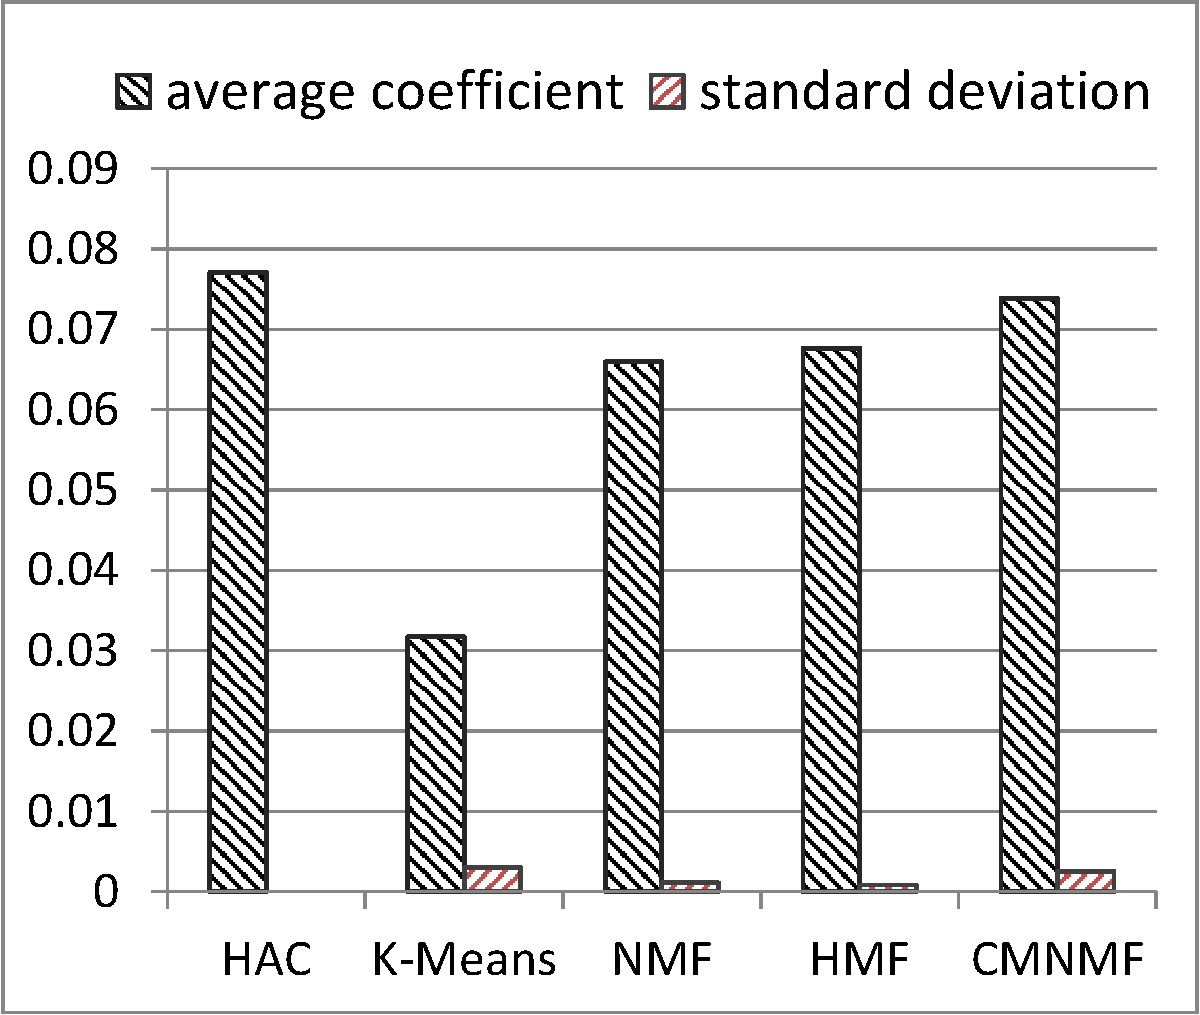
\includegraphics[width=\linewidth]{fig/jaccard.pdf}
    \centerline{(a)}
  \end{minipage}
  \begin{minipage}{.45\linewidth}
   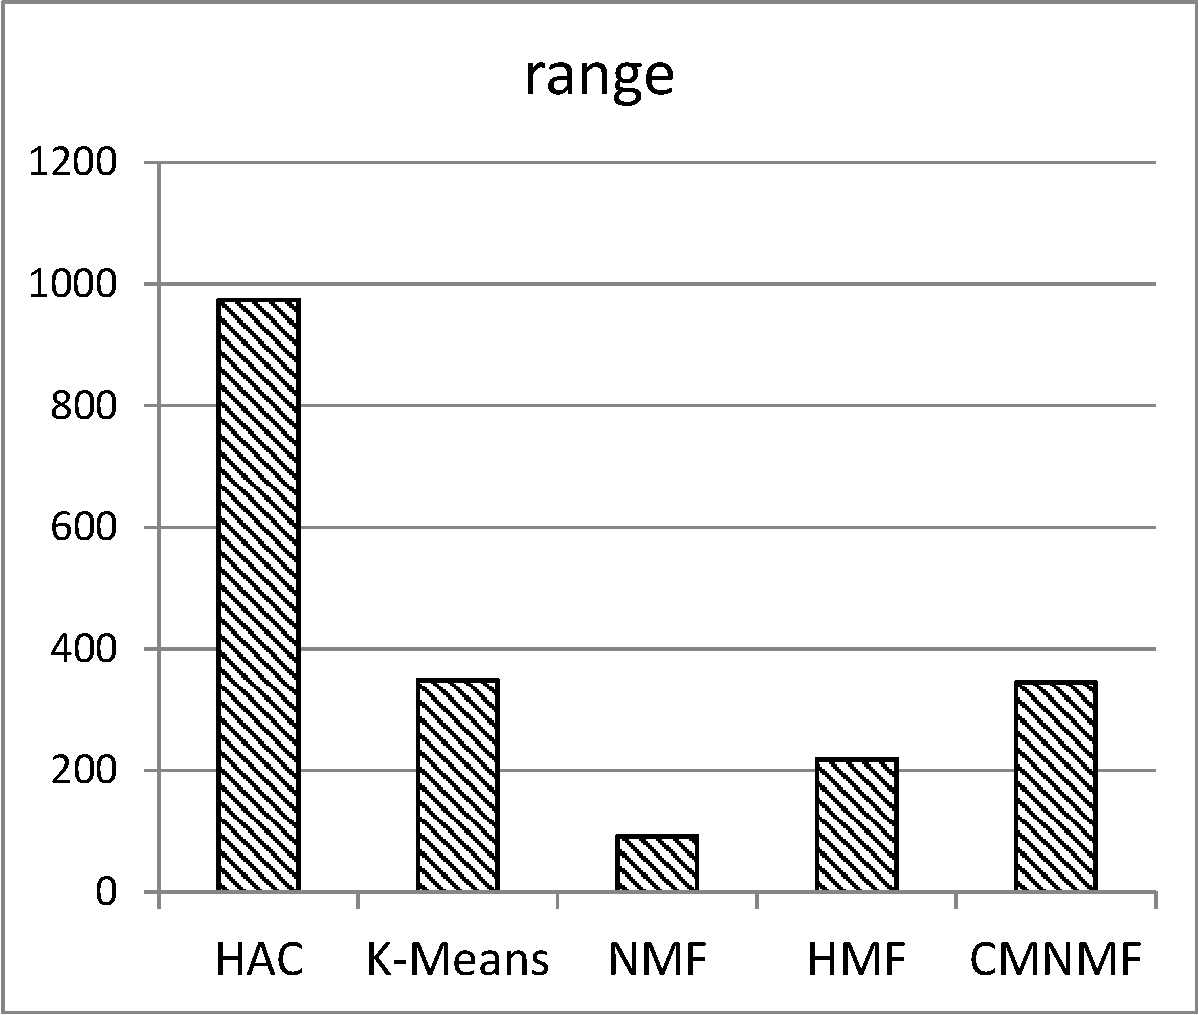
\includegraphics[width=\linewidth]{fig/range.pdf}
    \centerline{(b)}
  \end{minipage}
  \caption{(a) Comparative performance of the proposed method with various methods. (b) Range of gene clusters size of different methods.}
  \label{fig:jaccard}
\end{figure}

The $\alpha$ in our CMNMF model which balances the contributions from different levels is an important parameter. When $\alpha$ is close to 0, the model degenerates into NMF on level 4 and when $\alpha$ is big enough information from level 5 leads the model. The performance of CMNMF with different $\alpha$ is shown in Table \ref{tab:alpha_tune}. We can find that neither $\alpha$ is close to 0 nor big enough the CMNMF model performs best. When $\alpha$ is near 1, our method obtains a best performance which indicates that associations from different levels are mutual complementation with each other and our CMNMF model successfully captures this characteristic.
\begin{table}
\centering
\caption{Performance of CMNMF with different $\alpha$}
\label{tab:alpha_tune}
\begin{tabular}{|c||c|c|c|c|c|c|c|c|c|c|}
\hline
 $\alpha$ &0.1& 0.3&0.5&0.7&0.9&1&3&5&7&9\\
\hline
Jaccard coefficient& 0.056 & 0.059 & 0.066 & 0.063 & \textbf{0.071}& \textbf{0.074} & 0.062 & 0.053 & 0.050 & 0.049\\
\hline
\end{tabular}
\end{table}

\subsection*{4 parameter tuning}

\subsection*{5 Regularized CMNMF}

\subsection*{6 GO Enrichment Analysis on Gene Clusters}

We evaluate the biological significance of the identified gene clusters with GO (Gene Ontology) enrichment analysis by DAVID\cite{David}, an online functional annotation tool. It is adopted to analyze a set of genes with annotated gene ontologies in ``biological process''(BP) branch. In general, a large number of annotations means high-quality modules.

In our work, clusters with more than 300 genes and fewer than 5 genes are dropped as suggested in \cite{SMNMF}. Table \ref{tab:go} shows that modules identified by CMNMF have the most GO(BP) terms annotations under different p-value cutoff which demonstrates that our method can mine gene functional modules with more biological significance.

\begin{table}
\centering
\caption{Numbers of GO terms(BP) annotations in the modules under different p-value cutoff to consider a Go term(BP) enriched.}
\label{tab:go}
\begin{tabular}{|c||c|c|c|c|c|}
\hline
 &0.05 & 0.01& 0.001&0.0001&0.00001\\
\hline
\hline
K-Means&46  & 43& 39&38&32\\
\hline
NMF&2399 & 1996&1410&1016&769\\
\hline
HMF&1759& 1479&1030&729&520\\
\hline
CMNMF&\textbf{5586}& \textbf{4691}& \textbf{3594}&\textbf{2706}&\textbf{2090}\\
\hline
\end{tabular}
\end{table}

\section*{Conclusions}
In this paper, we introduce a consistent multiple nonnegative matrix factorization for data with hierarchical information. We first analyze the mechanism of our method on a simulated data, then compare the performance of CMNMF with other methods on mining gene modules. We conclude that the CMNMF method is an effective algorithm which can fully utilize the hierarchical structure information behind the data. Experiments on mining gene functional modules show the ability of CMNMF to identify modules with biological significance. In future, we will try to analyze the expansibility of CMNMF on more than just two levels and try to solve other tasks where data has a hierarchical structure.


%%%%%%%%%%%%%%%%%%%%%%%%%%%%%%%%%%%%%%%%%%%%%%
%%                                          %%
%% Backmatter begins here                   %%
%%                                          %%
%%%%%%%%%%%%%%%%%%%%%%%%%%%%%%%%%%%%%%%%%%%%%%

\begin{backmatter}

\section*{Competing interests}
  The authors declare that they have no competing interests.

\section*{Author's contributions}
    Text for this section \ldots

\section*{Acknowledgements}
This work is supported by the National Natural Science Foundation of China (No. 61300166 and No. 61105049), the Open Project Foundation of Information Technology Research Base of Civil Aviation Administration of China (CAAC-ITRB-201303 and CAAC-ITRB-201408), the Natural Science Foundation of Tianjin (No. 14JCQNJC00600), and the Science and Technology Planning Project of Tianjin (No. 13ZCZDGX01098).

%%%%%%%%%%%%%%%%%%%%%%%%%%%%%%%%%%%%%%%%%%%%%%%%%%%%%%%%%%%%%
%%                  The Bibliography                       %%
%%                                                         %%
%%  Bmc_mathpys.bst  will be used to                       %%
%%  create a .BBL file for submission.                     %%
%%  After submission of the .TEX file,                     %%
%%  you will be prompted to submit your .BBL file.         %%
%%                                                         %%
%%                                                         %%
%%  Note that the displayed Bibliography will not          %%
%%  necessarily be rendered by Latex exactly as specified  %%
%%  in the online Instructions for Authors.                %%
%%                                                         %%
%%%%%%%%%%%%%%%%%%%%%%%%%%%%%%%%%%%%%%%%%%%%%%%%%%%%%%%%%%%%%

% if your bibliography is in bibtex format, use those commands:
\bibliographystyle{bmc-mathphys} % Style BST file (bmc-mathphys, vancouver, spbasic).
\bibliography{bmc_article}      % Bibliography file (usually '*.bib' )
% for author-year bibliography (bmc-mathphys or spbasic)
% a) write to bib file (bmc-mathphys only)
% @settings{label, options="nameyear"}
% b) uncomment next line
%\nocite{label}

% or include bibliography directly:
% \begin{thebibliography}
% \bibitem{b1}
% \end{thebibliography}

%%%%%%%%%%%%%%%%%%%%%%%%%%%%%%%%%%%
%%                               %%
%% Figures                       %%
%%                               %%
%% NB: this is for captions and  %%
%% Titles. All graphics must be  %%
%% submitted separately and NOT  %%
%% included in the Tex document  %%
%%                               %%
%%%%%%%%%%%%%%%%%%%%%%%%%%%%%%%%%%%

%%
%% Do not use \listoffigures as most will included as separate files

\section*{Figures}
  \begin{figure}[h!]
  \caption{\csentence{Sample figure title.}
      A short description of the figure content
      should go here.}
      \end{figure}

\begin{figure}[h!]
  \caption{\csentence{Sample figure title.}
      Figure legend text.}
      \end{figure}

%%%%%%%%%%%%%%%%%%%%%%%%%%%%%%%%%%%
%%                               %%
%% Tables                        %%
%%                               %%
%%%%%%%%%%%%%%%%%%%%%%%%%%%%%%%%%%%

%% Use of \listoftables is discouraged.
%%
\section*{Tables}
\begin{table}[h!]
\caption{Sample table title. This is where the description of the table should go.}
      \begin{tabular}{cccc}
        \hline
           & B1  &B2   & B3\\ \hline
        A1 & 0.1 & 0.2 & 0.3\\
        A2 & ... & ..  & .\\
        A3 & ..  & .   & .\\ \hline
      \end{tabular}
\end{table}

%%%%%%%%%%%%%%%%%%%%%%%%%%%%%%%%%%%
%%                               %%
%% Additional Files              %%
%%                               %%
%%%%%%%%%%%%%%%%%%%%%%%%%%%%%%%%%%%

\section*{Additional Files}
  \subsection*{Additional file 1 --- Sample additional file title}
    Additional file descriptions text (including details of how to
    view the file, if it is in a non-standard format or the file extension).  This might
    refer to a multi-page table or a figure.

  \subsection*{Additional file 2 --- Sample additional file title}
    Additional file descriptions text.


\end{backmatter}
\end{document}
